\documentclass[a4paper,10pt]{article}
\usepackage[utf8]{inputenc}
\usepackage{mathtools}
\usepackage{amsthm}
\usepackage{amsmath}
\usepackage{amssymb}
\usepackage{mathabx}
\usepackage{proof}
\usepackage[textwidth=2cm,textsize=small]{todonotes}
\usepackage{hyperref}
\usepackage{bussproofs}
\usepackage{ifthen}

% TIKZ 
\usepackage{tikz}
\usetikzlibrary{positioning}
\usetikzlibrary{arrows,automata,backgrounds,decorations}
\usetikzlibrary{fadings}
\usetikzlibrary{shapes.geometric}
\usetikzlibrary{intersections}
\usetikzlibrary{shapes.multipart}
\usepgflibrary{decorations.pathreplacing} 
\usetikzlibrary{arrows,calc,topaths}
\usepackage{tikz-3dplot}
\tikzstyle{small}=[font=\footnotesize]
\tikzset{
    every picture/.style={>=stealth,auto,node distance=2cm},
}
% end TIKZ

%TODO STUFF
\newcommand{\filip}[1]{\todo[color=green!30]{{\bf Filip:} #1}}
\newcommand{\ifilip}[1]{\todo[inline, color=green!30]{{\bf Filip:} #1}}

\newtheorem{theorem}{Theorem}
\newtheorem{lemma}{Lemma}
\newtheorem{conjecture}{Conjecture}

\begin{document}
In this post we will reduce parity games to satisfiability of SMT formulas. We show to check satisfiability of these formulas by designing a proof system with resolution-like rules. Our first attempt will give a polynomial time algorithm (yay) that is not correct on all instances (dayum). In our second attempt we fix this providing a proof system that we conjecture works on all instances (yay) but in exponential time (dayum).

A short reminder: the existential player is called Eve and her nodes are circles; the universal player is Adam and his nodes are squares. We consider the variant of parity games where the objective for Eve is to win from all starting positions (it is equivalent to the usual setting). The instance of a parity game is denoted $\mathcal{P}$ and the set of its nodes is $V$.
Let $n$ be the number of all nodes in the parity game and let $d$ be the highest priority. W.l.o.g. we will assume that $d$ is odd. The theory in which we encode the formulas will have $\frac{d}{2}$ relations $>_i$ on $V$ for all odd indices $i \in \{1,3,\ldots,d\}$. These relations satisfy the following conditions:
\begin{itemize}
 \item $>_i \; \subseteq \; V \times V$ is a strict partial order (i.e., its transitive and antisymmetric);
 \item $>_i \; \subseteq \; >_{i+2}$ 
\end{itemize}
The non-strict variants $\ge_i$ are defined in the obvious way. \filip{does this require a comment that elements can be equal in the orders?}

We write how to build the formula for any parity game at the same time doing it on a real example (below). The formula we build should be obvious to understand for anyone familiar with the progress measure/the other name. 
\begin{center}
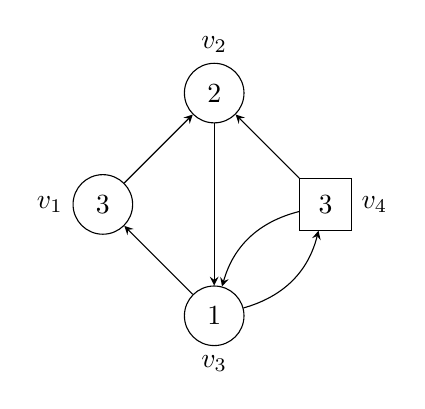
\begin{tikzpicture}[square/.style={regular polygon,regular polygon sides=4}]
\node[state,minimum size=5ex,label=left:{$v_1$}] (v1) {$3$};
\node[state,minimum size=5ex,above right of = v1,label=above:{$v_2$}] (v2) {$2$};
\node[state,minimum size=5ex,below right of = v1,label=below:{$v_3$}] (v3) {$1$};
\node[draw=black,square,minimum size=5ex,below right of=v2,label=right:{$v_4$}] (v4) {$3$};

\path (v1) edge[->] (v2)
(v2) edge[->] (v3)
(v3) edge[->] (v1)
(v3) edge[->,bend right] (v4)
(v4) edge[->,bend right] (v3)
(v4) edge[->] (v2)
;
\end{tikzpicture}
\end{center}\filip{Marcin said even players should be square and odd players triangle because it makes more sense, you can change it if you prefer}

Given a parity game $\mathcal{P}$ we construct the formula $\varphi_{\mathcal{P}}$.
For every node in the game we add one ore more clauses and the final formula is a conjunction of all these clauses. For every node $v$ of parity $i$ we define the clauses as follows.
\begin{itemize}
 \item If $v$ is owned by Adam then for every outgoing edge $v \to w$ we add a clause $v \succ w$, where $\succ$ is $>_i$ if $i$ is odd and $\ge_{i+2}$ otherwise.
 \item If $v$ is owned by Eve then we add one clause to $\varphi_\mathcal{P}$. For an outgoing edge $v \to w$ let $v \succ w$, where $\succ$ is $>_i$ if $i$ is odd and $\ge_{i+2}$ otherwise. We add a disjunct of all such clauses for every outgoing edge.
\end{itemize}

For the example parity game we obtain the following clauses:
\begin{align}
\begin{split}\label{eq:1}
&v_1 >_3 v_2 \\
&v_2 \ge_3 v_3 \\
&v_3 >_1 v_1 \vee v_3 >_1 v_4 \\
&v_4 >_3 v_2 \\
&v_4 >_3 v_3.
\end{split}
\end{align}

\begin{theorem}\label{theorem:formula}
The formula $\varphi_\mathcal{P}$ is satisfiable iff Eve wins the parity game from every node.
\end{theorem}
\begin{proof}
The proof follows from the progress measure formulation of parity games. We omit it here.
\end{proof}

\subsection{The first proof system}
From now on we will deal mostly with the satisfiability problem of the formula $\varphi_{\mathcal{P}}$. We call atoms the formulas $v >_i w$ or $v \ge_i w$ for all $i$.
We propose the proof system with three types of rules. For every disjunct of atoms $C$ (possibly $C$ is empty) and every odd $i \in \{1,3,\ldots,d\}$ we have the following rules
\begin{enumerate}
 \item Transitivity: \infer{C \vee v \ge_i v''}{
    C \vee v \ge_i v' & C \vee v' \ge_i v''
},\;\;
\infer{C \vee v >_i v''}{
    C \vee v \ge_i v' & C \vee v' >_i v''
}

\item Weakening: \infer{C \vee v \ge_i v'}{
    C \vee v >_i v'
},\;\;
\infer{C \vee v \ge_{i+2} v'}{
    C \vee v \ge_{i} v'
},\;\;
\infer{C \vee v >_{i+2} v'}{
    C \vee v >_{i} v'
}

\item Resolution: \infer{C \vee C'}{
    C \vee v \ge_i v' & C' \vee v' >_i v
}
\end{enumerate}
Let $S_{\mathcal{P}}$ be the set of clauses in $\varphi_{\mathcal{P}}$.
\begin{lemma}
\label{lemma:correctness}
If by applying rules (1)--(3) to $S_{\mathcal{P}}$ one can obtain the empty clause then Eve loses the parity game.
\end{lemma}
\begin{proof}
The proof follows from the assumption that $>_i$ and $\ge_i$ are partial orders and Theorem~\ref{theorem:formula}.
\end{proof}

It is tempting to state the converse implication, unfortunately it is not true. In the next section we will show a counterexample and how to extend this proof system to be complete. First, let us show how to obtain the empty clause from the example~\eqref{eq:1}, proving that Eve loses that game. For readability we write next to each non-atomic clause from which rule it is inferred.

\begin{prooftree}
\AxiomC{$v_3 >_1 v_1 \vee v_3 >_1 v_4$}
\UnaryInfC{$v_3 >_1 v_1 \vee v_3 >_3 v_4$ (2)}
\AxiomC{$v_4 >_3 v_3$}
\BinaryInfC{$v_3 >_1 v_1$ (3)}
\UnaryInfC{$v_3 >_3 v_1$ (2)}
\AxiomC{$v_1 >_3 v_2$}
\AxiomC{$v_2 \ge_3 v_3$}
\BinaryInfC{$v_1 >_3 v_3$ (1)}
\UnaryInfC{$v_1 \ge_3 v_3$ (2)}
\BinaryInfC{$\emptyset$ (3)}
\end{prooftree}

Now, let us explain that this proof system applied to parity games will work in polynomial time. First, observe that a parity game $\mathcal{P}$ can be turned into an equivalent game, where each node has at most two outgoing edges (by introducing polynomially many auxiliary nodes). Then by construction of $\varphi_{\mathcal{P}}$ each clause will be of width at most two, that is, either an atom or a disjunction of two atoms. Observe that applying rules (1)--(3) to such clauses we obtain clauses that are also of width two. Hence starting from the set of clauses $S_{\mathcal{P}}$ we can add a new clause only polynomially many times. It yields a polynomial algorithm.

\subsection{A counterexample and the complete proof system}

We show a parity game that shows that the converse of Lemma~\ref{lemma:correctness} is not true. The parity game is quite simple, there are five nodes $v_i$ for $i = 0,\ldots,4$. All nodes belong to Eve and all nodes have parity 1 (hence Eve loses the game). The edges are $v_i \to v_{i+1}$ and $v_i \to v_{i + 2}$ for all $i$, where $i+1$ and $i+2$ are calculated modulo 5.

\begin{center}
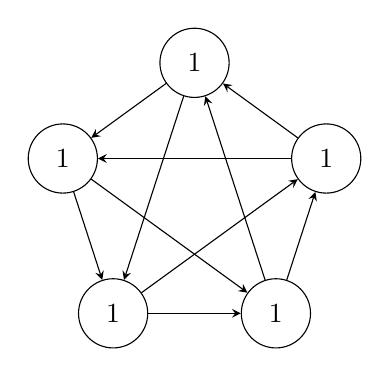
\begin{tikzpicture}
\node[draw=none,minimum size=3.5cm,regular polygon,regular polygon sides=5] (a) {};

\foreach \x in {1,2,...,5}{
  \node[state] (v\x) at (a.corner \x) {$1$};
}

\path
(v1) edge[->] (v2)
(v1) edge[->] (v3)
(v2) edge[->] (v3)
(v2) edge[->] (v4)
(v3) edge[->] (v4)
(v3) edge[->] (v5)
(v4) edge[->] (v5)
(v4) edge[->] (v1)
(v5) edge[->] (v1)
(v5) edge[->] (v2)
;

\end{tikzpicture}
\end{center}

The set of clauses obtained from this example is
$$
\bigcup_{i=0}^{4} \{v_i >_1 v_{i+1} \vee v_i >_1 v_{i+2}\}.
$$
It is not hard to see that the only rule that can be applied is one of the Weakening rules to obtain non-strict equalities. Transitivity rules cannot be applied because no two clauses have the same atoms. Resolution rules cannot be applied because they require combining two clauses that provide a cycle of length 2 ($v \ge_i v'$ and $v' >_i v$ in the definition of the rule). It is not hard to see that in the counterexample there only cycles of length 3. To overcome this problem we extend the resolution rules with the rule
$$
\infer{C \vee C' \vee C''}{
    C \vee v \ge_i v' & C' \vee v' \ge_i v'' & C'' \vee v'' >_i v
}
$$
And similar rules capturing cycles of length 4,5, etc.

\begin{conjecture}
Applying rules in the extended proof system to $S_{\mathcal{P}}$ one can obtain the empty clause iff Eve loses the parity game.
\end{conjecture}
We do not focus on the proof mainly because it is technical. Notice that in this proof system even if the initial clauses are of width 2 then the new rule allows the clauses to grow. Hence we do not know if this can be solved in polynomial time. Let us see how to solve the counterexample for the previous proof system.

\begin{prooftree}
\AxiomC{$v_1 >_1 v_2 \vee v_1 >_1 v_3$}
\AxiomC{$v_3 >_1 v_4 \vee v_3 >_1 v_5$}
\AxiomC{$v_5 >_1 v_1 \vee v_5 >_1 v_2$}
\TrinaryInfC{$v_1 >_1 v_2 \vee v_3 >_1 v_4 \vee v_5 >_1 v_2$}
\end{prooftree}

\subsection{What now?}
We believe this could yield an interesting class of parity games.

\end{document}
